
\subsection{Normalization versus Standardisation}
Our initial assumption was to use normalization to scale the data between a
fixed range between -1 and 1 because we did not know if the data would follow a Guassian
distribution. After testing both normalization and standardization,
standardization proved to perform significantly better.
The problem with scaling all values between a fixed range is that huge
outliers use up a lot of the range available, which will result in
most of the data having very small differences in values between them.
This can affect the NNs ability to differentiate between the observations.

\Cref{fig:time-series-standardization-vs-normalization} show two different time series
scaled with both techniques
\begin{figure}[h!]
  \centering
  \caption{Effects of different scaling techniques on a dataset with huge outliers.}
  \label{fig:time-series-standardization-vs-normalization}
  \begin{subfigure}[b]{0.49\textwidth}
    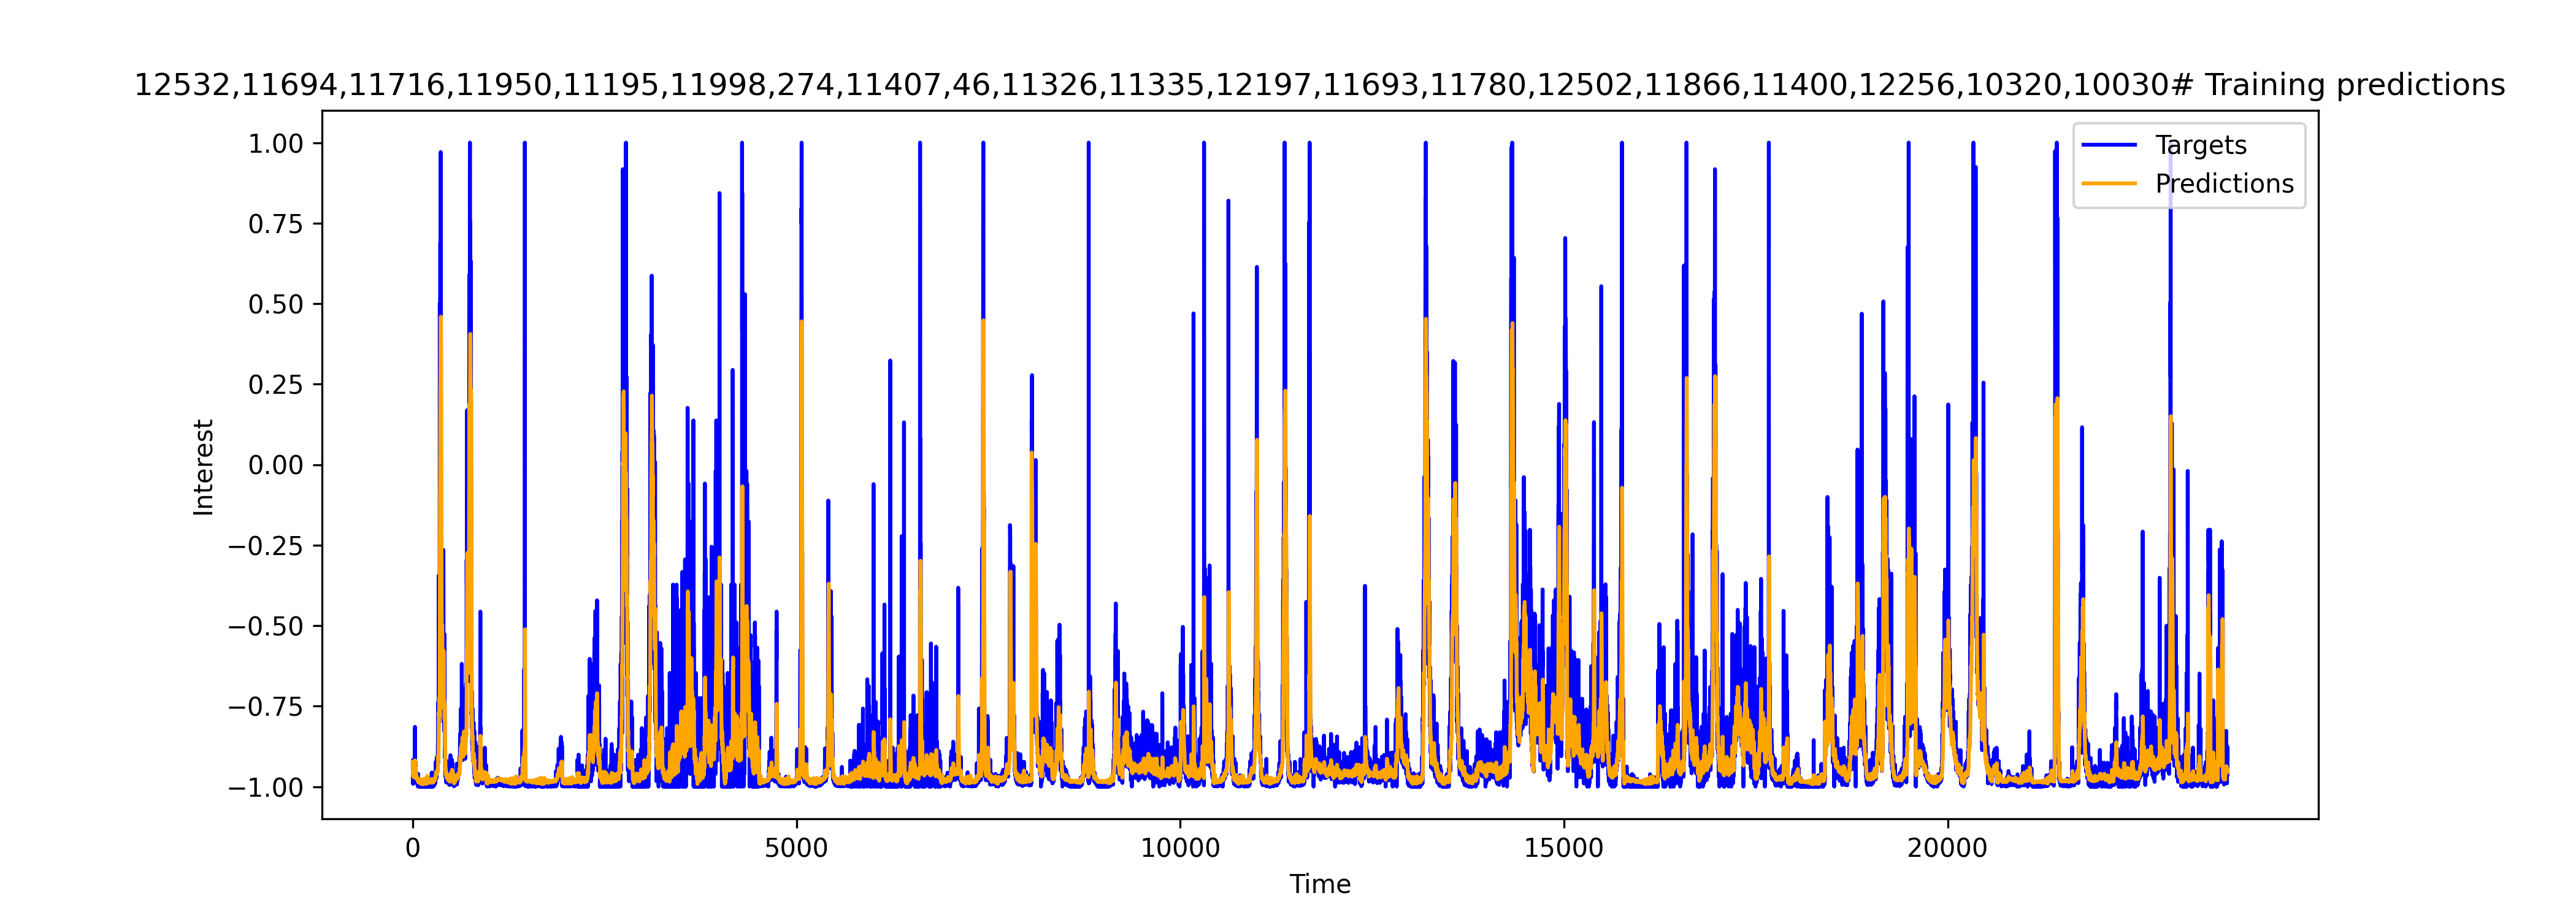
\includegraphics[width=\textwidth]{./figs/dataset/time-series_scaled_normalization2.png}
    \hfill
    \caption{A time series with huge outliers scaled using normalization. Most values are squeezed between -1 and -0.75.}
    \label{fig:time-series-normalization}
  \end{subfigure}
  \begin{subfigure}[b]{0.49\textwidth}
    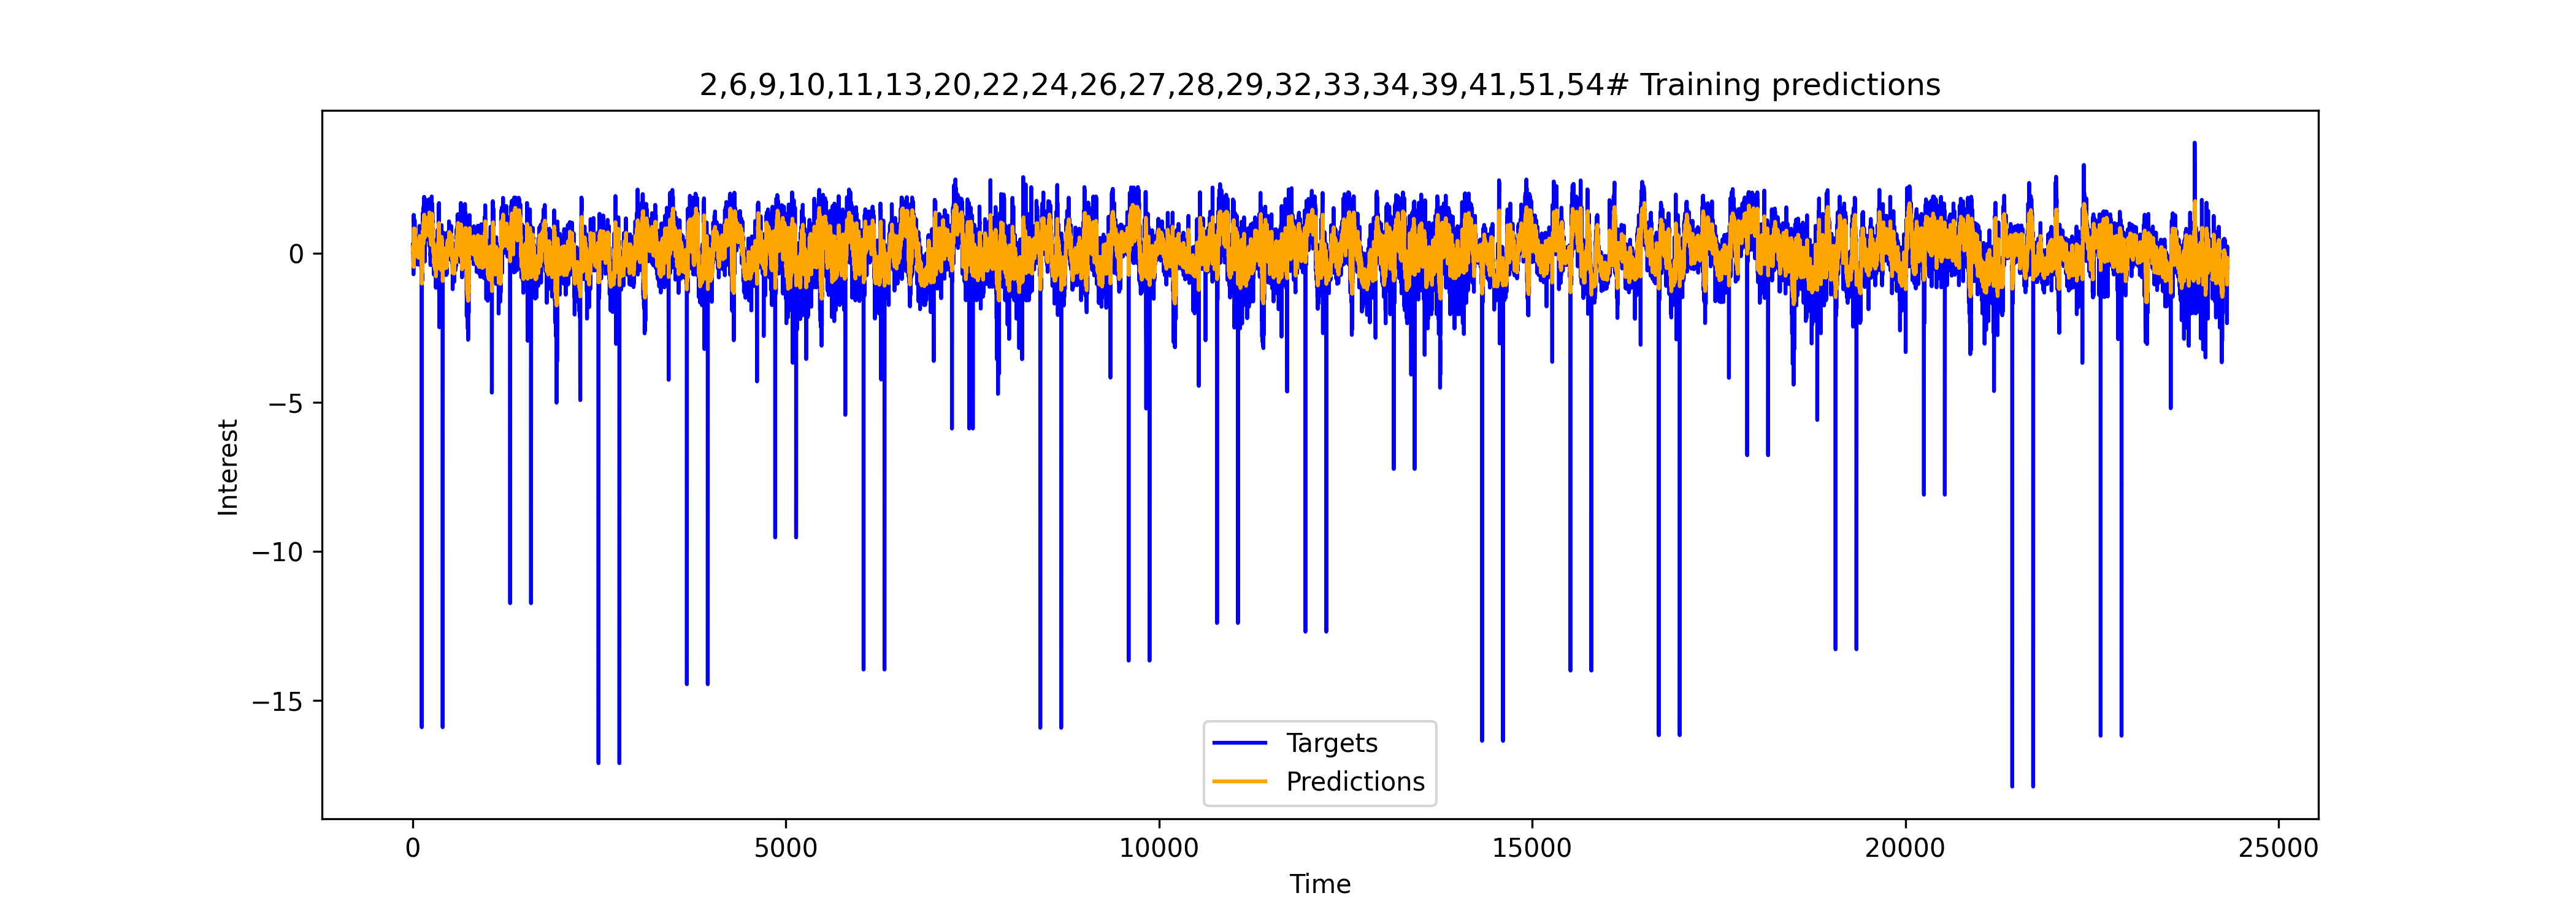
\includegraphics[width=\textwidth]{./figs/dataset/time-series_scaled_standardization.png}
    \hfill
    \caption{A time series scaled using standardization. Most values are centered between -2 and 2.}
    \label{fig:time-series-standardization}
  \end{subfigure}
\end{figure}